\documentclass{beamer}

\usepackage[utf8]{inputenc}
\usepackage{beamerthemesplit}
\usepackage{url}
\usepackage{hyperref}
\usepackage{tikz}
\usepackage{alltt}

\usepackage{listings}
\usepackage{marvosym}
\usepackage{color}
\usepackage[multidot]{grffile}
\usepackage{multirow}
\usepackage{array}
\usepackage{setspace}

\usetheme{Madrid}

\usecolortheme[RGB={132,186,75}]{structure}
\definecolor{cactusgreen}{RGB}{132,186,75}
\newcommand{\red}[1]{\textcolor{cactusgreen}{#1}}
\newcommand{\black}[1]{\textcolor{black}{#1}}

\graphicspath{{./pics/}}

\logo{
\includegraphics[height=0.7cm]{CLR_HOR}} 

\newcommand{\head}[2]
 {\frame{\frametitle{}\begin{centering}\LARGE#1\\#2\end{centering}}}

\newcommand{\abspic}[4]
 {\vspace{ #2\paperheight}\hspace{ #3\paperwidth}\includegraphics[height=#4\paperheight]{#1}\\
  \vspace{-#2\paperheight}\vspace{-#4\paperheight}\vspace{-0.0038\paperheight}}

\newcommand{\picw}[4]{{
 \usebackgroundtemplate{
 \color{black}\vrule width\paperwidth height\paperheight\hspace{-\paperwidth}\hspace{-0.01\paperwidth}
 \hspace{#4\paperwidth}\includegraphics[width=#3\paperwidth, height=\paperheight]{#1}}\logo{}
 \frame[plain]{\frametitle{#2}}
}}
\newcommand{\pic}[2]{\picw{#1}{#2}{}{0}}

\newcommand{\question}[1]{\frame{\begin{centering}\Huge #1\\\end{centering}}}
\newcommand{\redidot}{\makebox[0mm]{\hphantom{i}\red{i}}{\i}}
\newcommand{\blackidot}{\makebox[0mm]{\hphantom{i}\black{i}}{\i}}

% We want to use the infolines outer theme because it uses so less space, but
% it also tries to print an institution and the slide numbers
% Therefore, we here redefine the footline ourselfes - mostly a copy & paste from
% /usr/share/texmf/tex/latex/beamer/themes/outer/beamerouterthemeinfolines.sty
\defbeamertemplate*{footline}{infolines theme without institution and slide numbers}
{
  \leavevmode%
  \hbox{%
  \begin{beamercolorbox}[wd=.25\paperwidth,ht=2.25ex,dp=1ex,center]{author in head/foot}%
    \usebeamerfont{author in head/foot}\insertshortauthor
  \end{beamercolorbox}%
  \begin{beamercolorbox}[wd=.5\paperwidth,ht=2.25ex,dp=1ex,center]{title in head/foot}%
    \usebeamerfont{title in head/foot}\insertshorttitle
  \end{beamercolorbox}%
  \begin{beamercolorbox}[wd=.25\paperwidth,ht=2.25ex,dp=1ex,center]{date in head/foot}%
    \usebeamerfont{date in head/foot}\insertshortdate{}
  \end{beamercolorbox}}%
  \vskip0pt%
}
% No navigation symbols
\setbeamertemplate{navigation symbols}{}

\title[The Einstein Toolkit]{Introduction to the Einstein Toolkit}
\author[{Brandt and Others}]{Steven R. Brandt, Frank Löffler, Roland Haas, Peter Diener, others}
\institute{Center for Computation and Technology\\Louisiana State University, Baton Rouge, LA}
%\titlegraphic{\includegraphics[height=1.5cm]{einstein_flip}\\}
\date[2020-08-03]{Aug 3, 2020}

\begin{document}

\frame{\titlepage}

\frame{\frametitle{In the beginning...}
1.3 Billion Years Ago, two black holes, each with about 30 solar masses, collided. They released three solar masses worth of mass energy as gravitational waves. Earth is in the Proterozoic Eon. Life consists of eukaryotes, including multicellular life forms.
}

\frame{\frametitle{In the beginning...}
541 Million Years Ago, Phanerozoic Eon begins, complex life, including vertebrates, appears.
}

\frame{\frametitle{In the beginning...}
1 Million Years Ago, Neanderthals appear.
}

\frame{\frametitle{In the beginning...}
200 Thousand Years Ago, ``Anatomically Modern Humans" appear.
}

\frame{\frametitle{In the beginning...}
In 1687, Newton publishes ``Philosophiæ Naturalis Principia Mathematica"
}

\frame{\frametitle{In the beginning...}
In 1905, Einstein publishes his paper on special relativity.
}

\frame{\frametitle{In the beginning...}
In 1915, Einstein publishes his papers on general relativity.
}

\frame{\frametitle{In the beginning...}
In 1916, Schwarzchild publishes the Schwarzchild black hole solution
}

\frame{\frametitle{In the beginning...}
In 1936, Einstein correctly describes gravitational waves
}

\frame{\frametitle{In the beginning...}
In 1956, Felix Pirani eliminates coordinate confusion and describes gravitational waves using curvature
}

\frame{\frametitle{In the beginning...}
In 1963, Kerr publishes the Kerr black hole solution
}

\frame{\frametitle{In the beginning...}
In 1994, The head-on collision of two black holes was simulated, as well as distorted single black holes
}

\frame{\frametitle{In the beginning...}
In 1995, Distorted Kerr solutions were simulated by me. :)
}

\frame{\frametitle{In the beginning...}
In 1997, Cactus was created by Paul Walker and Joan Masso.
It remains as one of the best, completely open source, collaborative
frameworks for studying numerical relativity.
}

%\frame{\frametitle{In the beginning...}
%In 1999: Cactus 4.0: "Cactus Einstein" thorns
%In 1999-2002: EU Network develops the Whisky Code
%}

\frame{\frametitle{In the beginning...}
In 2005, Franz Praetorius published his results on evolving binary black hole spacetimes.
}

%\frame{\frametitle{In the beginning...}
%In 2007-2009: LSU/RIT/PennState/Caltech/GeorgiaTech/AEI collaborations
%}

\frame{\frametitle{In the beginning...}
In 2012: The Einstein Toolkit is created.
}

\frame{\frametitle{In the beginning...}
In 2015, LIGO detected gravitational waves from two black holes that collided 1.3 billion years ago. The event was called GW150914.
}

\frame{\frametitle{In the beginning...}
Oh man, look at those cavemen go...

  --- David Bowie
}

\frame{\frametitle{In the beginning...}
\abspic{cavemen}{-0.2}{.105}{0.63}
}

%In the late nineteen nineties, we knew that LIGO was going to happen--or, at least, most of us believed it would. But we weren't sure whether we could interpret the data LIGO would see.
%}

\frame{\frametitle{Einstein Toolkit}
 \abspic{einstein}{-0.2}{0.6}{0.23}
% \abspic{people/frank}    {0.55}{0.2  }{0.13}
 \abspic{people/sbrandt}  {0.55}{0.12 }{0.13}
 %\abspic{people/tanja}    {0.55}{0.302}{0.13}
 \abspic{people/diener}   {0.55}{0.205}{0.13}
 \abspic{people/roland}   {0.55}{0.275}{0.13}
 \abspic{people/helvi}   {0.55}{0.35}{0.13}
 \abspic{people/zach}   {0.55}{0.43}{0.13}
 %\abspic{people/ian}      {0.55}{0.455}{0.13}
 \abspic{people/bruno}    {0.55}{0.505}{0.13}
 %\abspic{people/christian}{0.55}{0.555}{0.13}
 \abspic{people/erik}     {0.55}{0.60}{0.13}
 \scriptsize
 \begin{itemize}
   \item Collection of scientific software components and tools to simulate and analyze general relativistic astrophysical systems
  \item Freely available as open source at \href{http://einsteintoolkit.org}{http://einsteintoolkit.org}
  \item Supported by {\tiny NSF 1550551/1550461/1550436/1550514, NSF 1212401/1212426/1212433/1212460, NSF 0903973/0903782/0904015 (CIGR), 0701566/0855892 (XiRel), 0721915 (Alpaca), 0905046/0941653(PetaCactus/PRAC)}
  \item State-of-the-art set of tools for numerical relativity, open source
  \item Currently 259 members from 172 sites and 39 countries
  \item $>200$ publications, $>30$ theses building on these components (as of 2013)
  \item Regular, tested releases
  \item User support through various channels
 \end{itemize}
}

\frame{\frametitle{Einstein Toolkit}
 \abspic{gw-waves}{-.1}{.45}{.20}
 \abspic{rhaas-pic}{.1}{.5}{.10}
 \abspic{colors}{.2}{.3}{.30}
 \abspic{nstar}{.2}{.5}{.20}
 \abspic{ebent}{.2}{.75}{.20}
 \abspic{twostars}{.4}{.3}{.20}
 \abspic{zachstar}{.4}{.7}{.20}
 \abspic{ruizstar}{-.1}{.7}{.20}
Science
\begin{itemize}
\item Binary Black Hole Mergers
\item Neutron Star Mergers
\item Supernovae
\item Accretion Disks
\item Boson Stars
\item Hairy Black Holes
\item Cosmic Censorship
\end{itemize}
}

\question{\vspace{1cm}Community Effort!\\\vspace{1cm}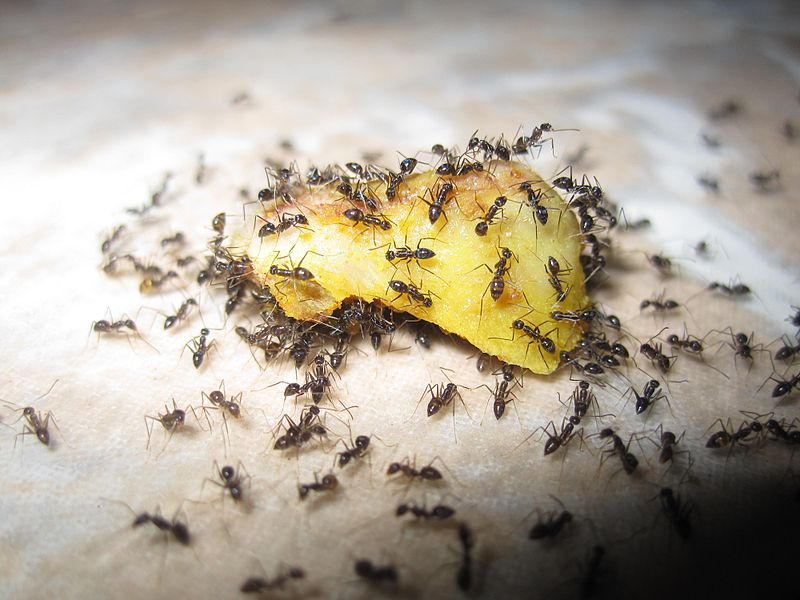
\includegraphics[width=4cm]{800px-Ants_eating_fruit}\vspace{1cm}}

\question{Why?}

\question{Computat{\redidot}onal Challenges\\
          \vspace{1cm}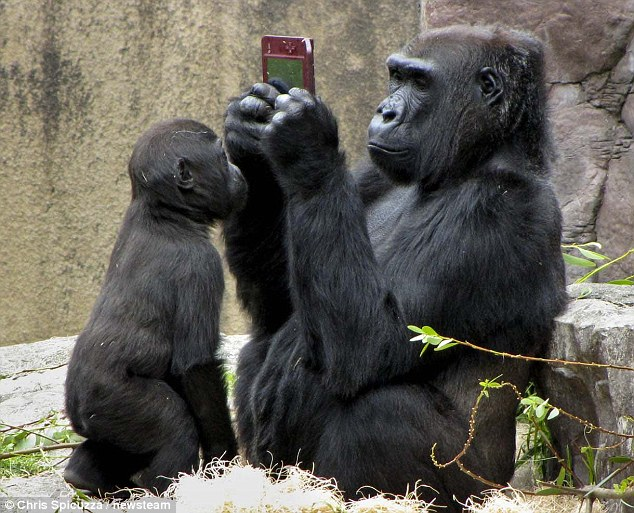
\includegraphics[width=4cm]{gorilla_tablet}}
\question{\red{Computat{\blackidot}onal} Challenges\\
          \vspace{1cm}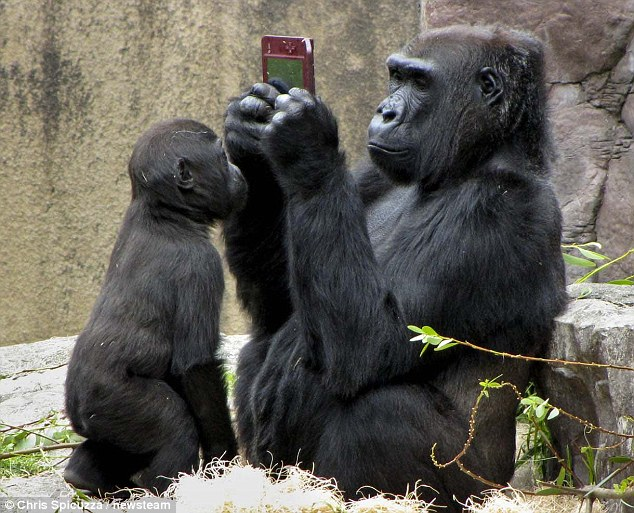
\includegraphics[width=4cm]{gorilla_tablet}}

\picw{Chinese-abacus}{}{1}{0}
%\pic{book_and_screen}{}
%\pic{8GB_vs_8Byte}{}

\frame{\frametitle{More and more diverse hardware}
 %\abspic{05_intel_ivy_bridge}         {-0.20}{0.0}{0.3}
 %\abspic{07_Nvidia_tesla_k10}         {-0.05}{0.4}{0.3}
 %\abspic{10_KnightsCornerChip_in_hand}{ 0.10}{0.7}{0.25}
 \abspic{arm}{-0.20}{0.0}{0.3}
 \abspic{icore9}{-0.25}{0.4}{.3}
 \abspic{radeon}{.15}{.1}{.3}
 \abspic{nvidia}{.10}{.4}{.3}
}
\picw{fugaku}{}{1}{0}
\picw{borg}{}{1}{0}

\frame{\frametitle{Computational Challenges}
 \abspic{640px-Gorilla_Scratching_Head}{0.2}{0.5}{0.35}
 \begin{itemize}
 \item Simulate cutting edge science
 \item Use latest numerical methods
 \item Make use of latest hardware
  \begin{itemize}
  \item Cache
  \pause
  \item Vector %(Kranc, NRPy+)
  \pause
  \item Scale to many cores %(openmp)
  \pause
  \item Scale to many nodes %(MPI, Carpet)
  \pause
  \item Algorithms %(Adaptive Mesh Refinement, Carpet)
  %\item GPU %(AMReX?)
  %\item FPGA?
  %\item Q-Bits?
  %\item Neuromorphic chips?
  \end{itemize}
 \end{itemize}
}


\frame[containsverbatim]{ \frametitle{Computational Challenges}
  \begin{itemize}
    \item Efficient use of all hardware is complex and tedious.
    \item Requires experts from different disciplines
    \item Requires good data layouts and APIs 
    \item To ensure correctness, need good modularization on
          a number of levels
          and understanding of advanced programming concepts.
    \item Design and implementation needs to be carefully thought out
	  in order to ensure extensibility and portability.
  \end{itemize}
}

%\frame[containsverbatim]{ \frametitle{Domain Decomposition}
%  \begin{minipage}[b]{6.5cm}
%    \begin{itemize}
%      \item In a domain decomposition scheme, the discrete elements (points,
%            cells, particles, \ldots) are distributed among the processors.
%      \item Each process handles only those that it \emph{owns} (without
%            requiring communication).
%      \item Accessing elements from neighboring processes requires
%            communication (e.g.\ at domain boundaries).
%    \end{itemize}
%  \end{minipage}
%  \raisebox{2.0em}{
%    \begin{minipage}[t]{4.5cm}
%      \includegraphics[width=4.3cm]{pics/wire-frame}
%    \end{minipage}
%  }
%}

\frame { \frametitle{Domain Decomposition}
 Without Ghostzones:\\
 \begin{centering}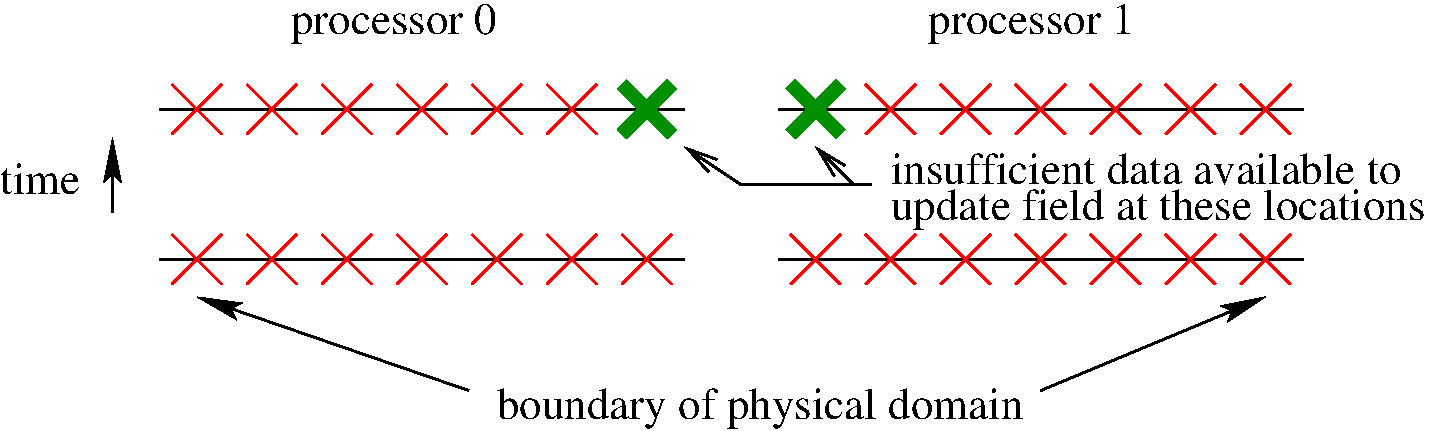
\includegraphics[width=9cm]{pics/1dnoghost}\\\end{centering}
 With Ghostzones:\\
 \begin{centering}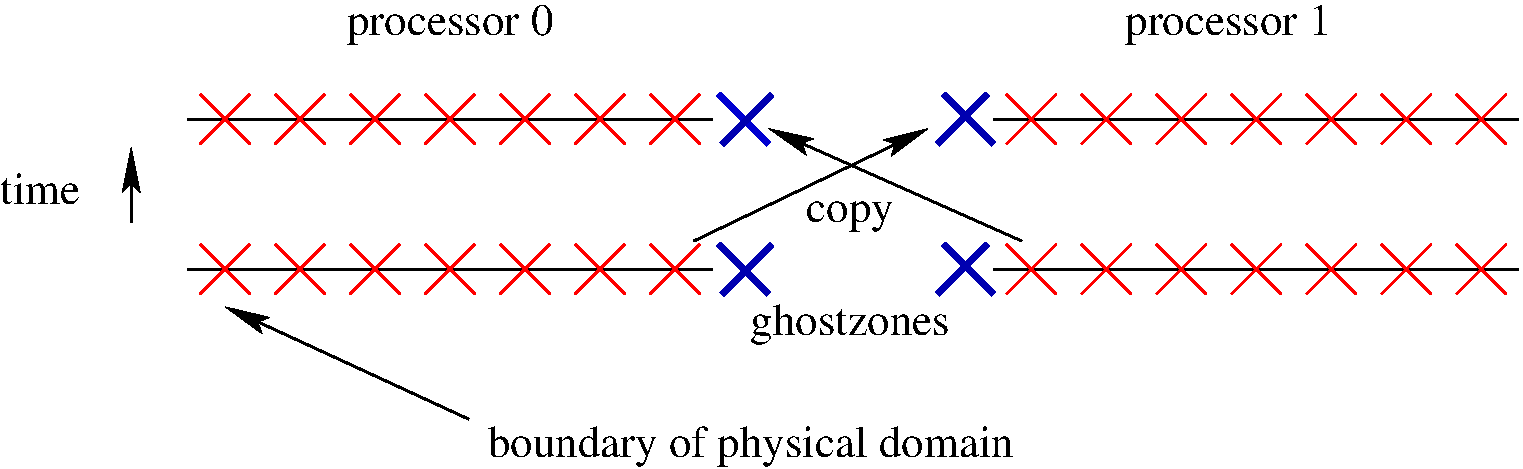
\includegraphics[width=9cm]{pics/withghost}\\\end{centering}
}

\frame { \frametitle{Domain decomposition}
 \begin{centering}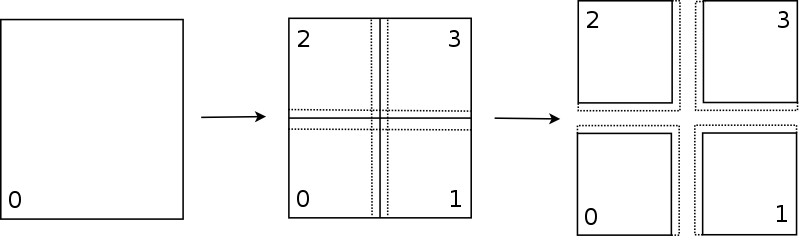
\includegraphics[width=11cm]{pics/domain_decomposition}\\\end{centering}
}
\frame { \frametitle{Multiblock and refinement}
 \begin{centering}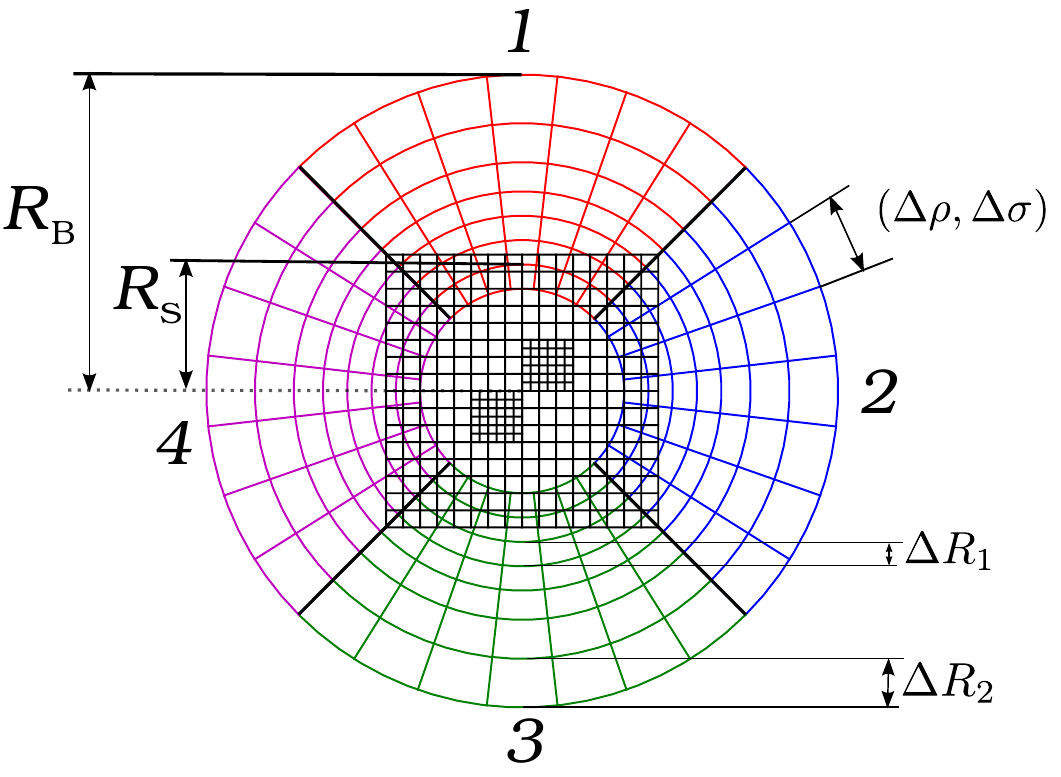
\includegraphics[width=11cm]{pics/multiblock}\\\end{centering}
}

\frame{\frametitle{Computational Challenges}
 \abspic{640px-Gorilla_Scratching_Head}{-0.1}{0.5}{0.35}
 \begin{itemize}
 \item Simulate cutting edge science
 \item Use latest numerical methods
 \item Make use of latest hardware
  \begin{itemize}
  %\item Cache
  \item Vector (Kranc, NRPy+)
  \pause
  \item Scale to many cores (openmp)
  \pause
  \item Scale to many nodes (MPI, Carpet, CarpetX)
  \pause
  \item Algorithms / AMR (Adaptive Mesh Refinement, Carpet, CarpetX, MOL)
  \pause
  \item GPU (CarpetX)
  \pause
  \item FPGA?
  \pause
  \item ASIC?
  \pause
  \item Neuromorphic processor?
  \pause
  \item Q-bits?
  \end{itemize}
 \end{itemize}
}

\frame{\frametitle{Computational Challenges}
 \abspic{640px-Gorilla_Scratching_Head}{-0.1}{0.5}{0.35}
More Mundane Challenges
\begin{itemize}
\pause
\item Efficient I/O
\pause
\item HDF5
\pause
\item Checkpoint/Restart
\pause
\item Parameter Parsing
\pause
\item Visualization
\pause
\item Steering
\end{itemize}
}

%\frame[containsverbatim]{ \frametitle{The Wave Equation}
%  Approximating the pressure $P(x,t)$ with a grid function $P_i^{(n)}$.
%  \begin{minipage}[b]{3.05cm}
%    \includegraphics[width=3cm]{pics/discretisation}
%  \end{minipage}
%  \raisebox{8em}{
%  \begin{minipage}[t]{8.5cm}
%    \begin{eqnarray}
%      \frac{\partial^2 P}{\partial t^2} & = & 
%       v^2\frac{\partial^2 P}{\partial x^2} \nonumber \\
%      & \Downarrow & \nonumber \\
%      \frac{P_i^{(n+1)}-2 P_i^{(n)}+P_i^{(n-1)}}{\Delta t^2} & = &
%      v^2\frac{P_{i+1}^{(n)}-2 P_i^{(n)}+P_{i-1}^{(n)}}{\Delta x^2} \nonumber
%    \end{eqnarray}
%  \end{minipage}}
%  The error from this time and space discretisation is $O(h^2)$.
%}

\question{Collaborat{\redidot}ve Challenges\\
          \vspace{1cm}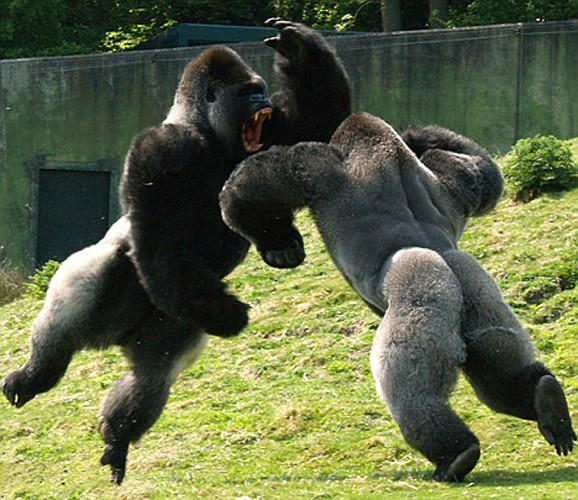
\includegraphics[width=4cm]{gorilla_fight}}
\question{\red{Collaborat{\blackidot}ve} Challenges\\
          \vspace{1cm}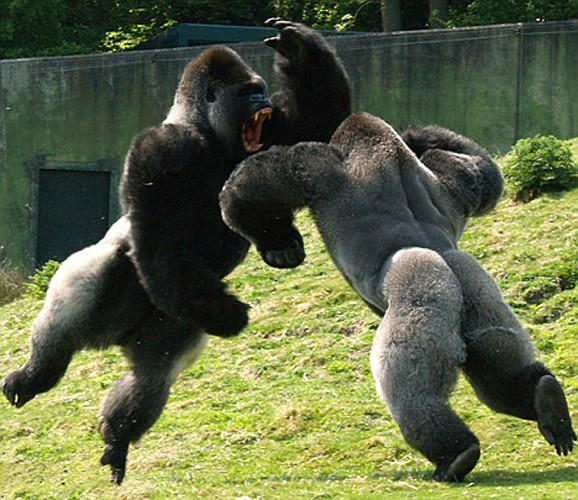
\includegraphics[width=4cm]{gorilla_fight}}

\frame{
  \abspic{community_only_problem}    {-0.1}{0.1}{0.6}
}

\frame{
  \abspic{community_with_problem}    {-0.1}{0.1}{0.6}
  \abspic{hurricane}     {-0.35}{0.05}{0.2}
  \abspic{wind_park}     {-0.30}{0.73}{0.2}
  \abspic{space_shuttle} { 0.20}{0.00}{0.2}
  \abspic{crab}          { 0.20}{0.75}{0.2}
}

\frame{
  \abspic{community_with_computation}{-0.1}{0.1}{0.6}
  \abspic{hurricane}     {-0.35}{0.05}{0.2}
  \abspic{wind_park}     {-0.30}{0.73}{0.2}
  \abspic{space_shuttle} { 0.20}{0.00}{0.2}
  \abspic{crab}          { 0.20}{0.75}{0.2}
  \abspic{bluewaters}        {-0.07}{0.40}{0.15}
  \abspic{tianhe1}       { 0.31}{0.40}{0.15}
}

\frame{
  \abspic{community_of_groups}       {-0.1}{0.1}{0.6}
  \abspic{hurricane}     {-0.35}{0.05}{0.2}
  \abspic{wind_park}     {-0.30}{0.73}{0.2}
  \abspic{space_shuttle} { 0.20}{0.00}{0.2}
  \abspic{crab}          { 0.20}{0.75}{0.2}
  \abspic{bluewaters}        {-0.07}{0.40}{0.15}
  \abspic{tianhe1}       { 0.31}{0.40}{0.15}
}

\frame{
  \abspic{community_of_groups}       {-0.1}{0.1}{0.6}
  \abspic{hurricane}     {-0.35}{0.05}{0.2}
  \abspic{wind_park}     {-0.30}{0.73}{0.2}
  \abspic{space_shuttle} { 0.20}{0.00}{0.2}
  \abspic{crab}          { 0.20}{0.75}{0.2}
  \abspic{email}         { 0.06}{0.38}{0.10}
  \abspic{phone}         { 0.04}{0.53}{0.10}
  \abspic{irc}           { 0.25}{0.40}{0.10}
  \abspic{www}           { 0.25}{0.55}{0.10}
}

\frame{
  \abspic{email}         { 0.06}{0.38}{0.10}
  \abspic{phone}         { 0.04}{0.53}{0.10}
  \abspic{irc}           { 0.25}{0.40}{0.10}
  \abspic{www}           { 0.25}{0.55}{0.10}
  \pause
  \abspic{Subversion-logo}{-0.28}{0.20}{0.23}
  \abspic{Git-logo}       {-0.20}{0.40}{0.13}
  \abspic{Mercurial_logo} {-0.20}{0.70}{0.13}
  \pause
  \abspic{Trac_logo}      { 0.10}{0.05}{0.10}
  \pause
  \abspic{Mediawiki_logo} { 0.10}{0.70}{0.15}
  \pause
  \abspic{Workshop}       { 0.35}{0.10}{0.05}
}

\frame{
  \abspic{community_with_problems}   {-0.1}{0.1}{0.6}
  \abspic{hurricane}     {-0.35}{0.05}{0.2}
  \abspic{wind_park}     {-0.30}{0.73}{0.2}
  \abspic{space_shuttle} { 0.20}{0.00}{0.2}
  \abspic{crab}          { 0.20}{0.75}{0.2}
}

\frame{
  \abspic{community_with_competition}{-0.1}{0.1}{0.6}
  \abspic{crab}          {-0.35}{0.05}{0.2}
  \abspic{crab}          {-0.30}{0.73}{0.2}
  \abspic{crab}          { 0.20}{0.00}{0.2}
  \abspic{crab}          { 0.20}{0.75}{0.2}
}

\frame{
  \abspic{community_with_standards}{-0.1}{0.1}{0.6}
  \abspic{hurricane}     {-0.35}{0.05}{0.2}
  \abspic{wind_park}     {-0.30}{0.73}{0.2}
  \abspic{space_shuttle} { 0.20}{0.00}{0.2}
  \abspic{crab}          { 0.20}{0.75}{0.2}
}

\frame{
  \abspic{community_with_standards}{-0.1}{0.1}{0.6}
  \abspic{hurricane}     {-0.35}{0.05}{0.2}
  \abspic{wind_park}     {-0.30}{0.73}{0.2}
  \abspic{space_shuttle} { 0.20}{0.00}{0.2}
  \abspic{crab}          { 0.20}{0.75}{0.2}
  \abspic{Imperial-Metric}{0.35}{0.40}{0.12}
  \pause
  \abspic{hdf_logo}      {-0.10}{0.45}{0.1}
}

\frame{
  \abspic{community_with_tools}{-0.1}{0.1}{0.6}
  \abspic{hurricane}     {-0.35}{0.05}{0.2}
  \abspic{wind_park}     {-0.30}{0.73}{0.2}
  \abspic{space_shuttle} { 0.20}{0.00}{0.2}
  \abspic{crab}          { 0.20}{0.75}{0.2}
}
\frame{
  \abspic{community_with_tools_examples}{-0.1}{0.1}{0.6}
}
\frame{
  \abspic{community_with_tools_examples}{-0.1}{0.1}{0.6}
  \abspic{Tux-linux_logo}     {-0.35}{0.05}{0.2}
  \abspic{Windows_logo}       {-0.30}{0.73}{0.2}
  \abspic{Apple_Logo}         { 0.20}{0.03}{0.15}
  \abspic{Tux-linux_logo}     { 0.17}{0.13}{0.2}
  \abspic{Apple_Logo}         { 0.24}{0.77}{0.15}
}

\frame{
  \abspic{community_with_credit}{-0.1}{0.1}{0.6}
  \abspic{hurricane}     {-0.35}{0.05}{0.2}
  \abspic{wind_park}     {-0.30}{0.73}{0.2}
  \abspic{space_shuttle} { 0.20}{0.00}{0.2}
  \abspic{crab}          { 0.20}{0.75}{0.2}
}
\frame{
  \abspic{community_with_credit}{-0.1}{0.1}{0.6}
  \abspic{crab}          {-0.35}{0.05}{0.2}
  \abspic{crab}          {-0.30}{0.73}{0.2}
  \abspic{crab}          { 0.20}{0.00}{0.2}
  \abspic{crab}          { 0.20}{0.75}{0.2}
}


\frame{\frametitle{Collaborative Challenges}
 \abspic{germany}              {-0.09}{0.36}{0.2}
 \abspic{germany_map}          { 0.12}{0.46}{0.2}
 \abspic{800px-Los_Angeles_Skyline_telephoto}{-0.05}{0.68}{0.2}
 \abspic{georgia}              { 0.26}{0.56}{0.18}
 \abspic{louisiana}            { 0.42}{0.37}{0.21}
 \abspic{neworleans}           { 0.45}{0.65}{0.18}
How can we work together?
\begin{itemize}
    \item Researchers in the USA
    \begin{itemize}
        \item Louisiana
        \item Illinois
        \item Virginia
        \item Pennsylvania
        \item Georgia
        \item California
    \end{itemize}
    \item Researchers in Other countries
    \begin{itemize}
        \item Italy
        \item Spain
        \item Portugal
        \item Canada
        \item Germany
    \end{itemize}
\end{itemize}
}

\frame{\frametitle{Einstein Toolkit}
 \abspic{einstein}{-0.2}{0.6}{0.23}
 \abspic{cactuslogo}{0.22}{0.20}{.11}
 \abspic{simfac-trim}{0.25}{0.32}{.15}
 \abspic{kranc-trim}{0.39}{0.20}{.11}
 \abspic{Nerpy}{0.5}{0.30}{.15}
\begin{columns}
\begin{column}{0.5\textwidth}
Goals:
\begin{itemize}
\item Community Driven
\item Core computational tool for GR
\item General purpose tool!
\end{itemize}
Components:
\begin{itemize}
\item Cactus
\item Simulation Factory
\item Kranc
\item NRPy+
\item Science Modules
\end{itemize}
\end{column}
\begin{column}{0.5\textwidth}
Guiding Principles
\begin{itemize}
\item Open
\item Community Driven
\item Good interfaces
\item Separation of physics
      from computational
      infrastructure
\item Code reviews
\end{itemize}
\end{column}
\end{columns}
}

\frame{\frametitle{Einstein Toolkit as growing project}
 \abspic{jigsaw1} {-0.082}{0.35}{0.16}
 \vspace{-4cm}
 \begin{itemize}
  \item \small Initially: some infrastructure, some application code
 \end{itemize}
}
\frame{\frametitle{Einstein Toolkit as growing project}
 \abspic{jigsaw2} {-0.2}{0.2}{0.4}
 \vspace{-4cm}
 \begin{itemize}
  \item \small Growing application suite
 \end{itemize}
}
\frame{\frametitle{Einstein Toolkit as growing project}
 \abspic{jigsaw3} {-0.2}{0.14}{0.52}
 \vspace{-4cm}
 \begin{itemize}
  \item \small Growing infrastructure ``return''
 \end{itemize}
}
\frame{\frametitle{Einstein Toolkit as growing project}
 \abspic{jigsaw4} {-0.205}{0.135}{0.525}
 \vspace{-4cm}
 \begin{itemize}
  \item \small Users from more fields of science
 \end{itemize}
}
\frame{\frametitle{Einstein Toolkit as growing project}
 \abspic{jigsaw5} {-0.205}{0.135}{0.525}
 \vspace{-4cm}
 \begin{itemize}
  \item \small Most modules open-source, but not necessarily all
 \end{itemize}
}

\question{Base Modules\\*[1em]
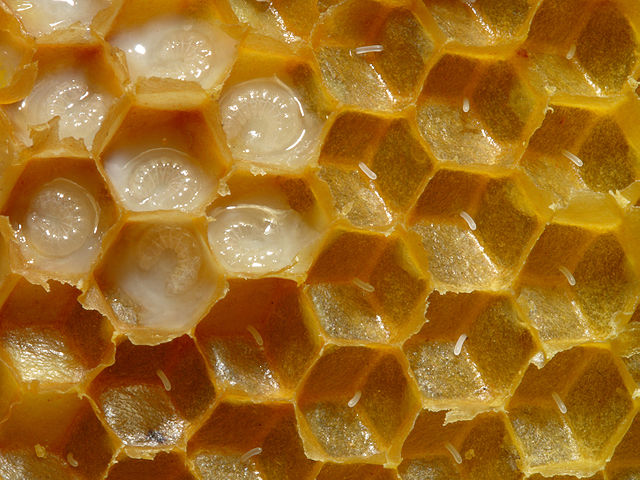
\includegraphics[width=0.4\textwidth]{640px-Bienenwabe_mit_Eiern_und_Brut_5}}

\frame{\frametitle{The Einstein Equations}
  \abspic{Eeq_Eeq}{-0.25}{0.0}{0.70}
}
\frame{
  \abspic{Eeq_curvature}{-0.25}{0.0}{0.70}
}
\frame{
  \abspic{Eeq_constants}{-0.25}{0.0}{0.70}
}
\frame{
  \abspic{Eeq_matter}{-0.25}{0.0}{0.70}
}
\frame{
  \abspic{Eeq_all}{-0.25}{0.0}{0.70}
}

\frame{
  \abspic{ET_layout_Eeq}{-0.25}{0.0}{0.70}
}
\frame{
  \abspic{ET_layout_ADMBase}{-0.25}{0.0}{0.70}
}
\frame{
  \abspic{ET_layout_Base2}{-0.25}{0.0}{0.70}
}
\frame{
  \abspic{ET_layout_Tmunu}{-0.25}{0.0}{0.70}
}
\frame{
  \abspic{ET_layout_inv_cowling}{-0.25}{0.0}{0.70}
}
\frame{
  \abspic{ET_layout_evolution}{-0.25}{0.0}{0.70}
}
\frame{
  \abspic{ET_layout_all}{-0.25}{0.0}{0.70}
}
\frame{
  \abspic{ET_layout_multiple}{-0.25}{0.0}{0.70}
}

\frame{\frametitle{Guiding Principles}
 \abspic{opensource_logo}{0.2}{0.7}{0.2}
 \begin{itemize}
  \item Open, community-driven software development
  \item Separation of \textbf{physics} software and \textbf{computational} infrastructure
  \item Stable interfaces, allowing extensions
  \item Simplify usage where possible:
   \begin{itemize}
    \item Doing science $>>$ Running a simulation
    \item Students need to know a lot about physics\\
           (meaningful initial conditions, numerical stability,\\
           accuracy/resolution, have patience, have curiosity,\\
           develop a ``gut feeling'' for what is right ...)
    \item Einstein Toolkit \textbf{cannot} give that, \textbf{however}:
    \item Open codes that are easy to use allow to concentrate on these things!
   \end{itemize}
 \end{itemize}
}

\frame{\frametitle{Credits, Citations}
 \abspic{barretr_Book.png}{0.2}{0.7}{0.2}
 In academics: citations, citations, citations!\\
 For Einstein Toolkit:
 \begin{itemize}
  \item Open and free source
  \item No \textbf{requirement} to cite anything
  \item However: \textbf{requested} to cite 
  \begin{itemize}
   \item The DOI doi:10.5281/zenodo.3866075
   \item Maybe the ET or Cactus papers
   \item Some papers for the components list a few as well
   \item List published on website and manage through publication database
  \end{itemize}
 \end{itemize}
}

\section{Vision}
\frame{\frametitle{Vision}
 \abspic{arrow}{0}{0.65}{0.2}
 Cutting Edge / Future
 \begin{itemize}
  %\item Inclusion of ``more physics'', e.g. general \\MHD, tabulated equations of state
  %\item Improve scaling of existing mesh methods
  \item New Driver Thorn: AMReX
  \item New Declarative Synchronization: Presync
  \item New Spherical Coordinates Thorn (RIT)
  \item New Python Code Generator: NRPy+
 \end{itemize}
 Recent
 \begin{itemize}
  \item Proca Thorns
  \item LEAN Thorns
  \item GiRaFFE thorns
 \end{itemize}
}

\section{Summary}
\frame{\frametitle{Summary}
 \abspic{people}    {-0.15}{0.55}{0.15}
 \abspic{opensource_logo}{0.05}{0.8}{0.1}
 \begin{centering}
  \href{run:mplayer -noaspect -fs -zoom -vo xv ../pics/Einstein_Toolkit.avi}{
    
\includegraphics[height=2cm]{cactuslogo}}\\
 \end{centering}
 {\large Einstein Toolkit\\}
 \begin{itemize}
  \item http://einsteintoolkit.org/
  \item Tools for high-performance computing in numerical relativity
  \item Open Source
  \item World-wide, open Community
  \item Used in high-end research
 \end{itemize}
}

\frame{\frametitle{Supported By}
The Einstein Toolkit has been supported by \\
NSF 2004157/2004044/2004311/2004879/2003893,\\
NSF 1550551/1550461/1550436/1550514,\\
NSF 1212401/1212426/1212433/1212460,\\
NSF 0903973/0903782/0904015 (CIGR), 0701566/0855892 (XiRel), 0721915 (Alpaca), 0905046/0941653(PetaCactus/PRAC). Any opinions, findings, and conclusions or recommendations expressed in this material are those of the author(s) and do not necessarily reflect the views of the National Science Foundation.
}


\end{document}

